\section{Related work} \label{releatedWork}
    
This section covers an overview of the material that can be seen as the direct foundation for this proposal.

\subsection{State model difference}
The \verb|StateModel.Difference| package, added by Ricós\cite{stateDiff}, offers a proof of concept for calculating differences between the state models. With this proof of concept, two inferred models are being compared with each other. For the comparison the \verb|abstractStateId| is being used. This is great for the proof of concept but due to the boolean nature of this comparison, the state either exist or not, it can result in many 'false' changes. 



Ricós difference algorithm\cite{stateDiff} outputs two classification of changes between two versions: added and removed state. Let $A$ be a set of \verb|abstractStateId|'s of version 1 of the SUT, let $B$ be a set of \verb|abstractStateId|'s of version 2 of the SUT. The removed states can be written as
\[A-B = \lbrace x | x \in A \wedge x \notin B \rbrace\]
the states that are added can be written as
\[B-A = \lbrace x | x \in B \wedge x \notin A \rbrace\]

\begingroup
\captionsetup{type=figure}
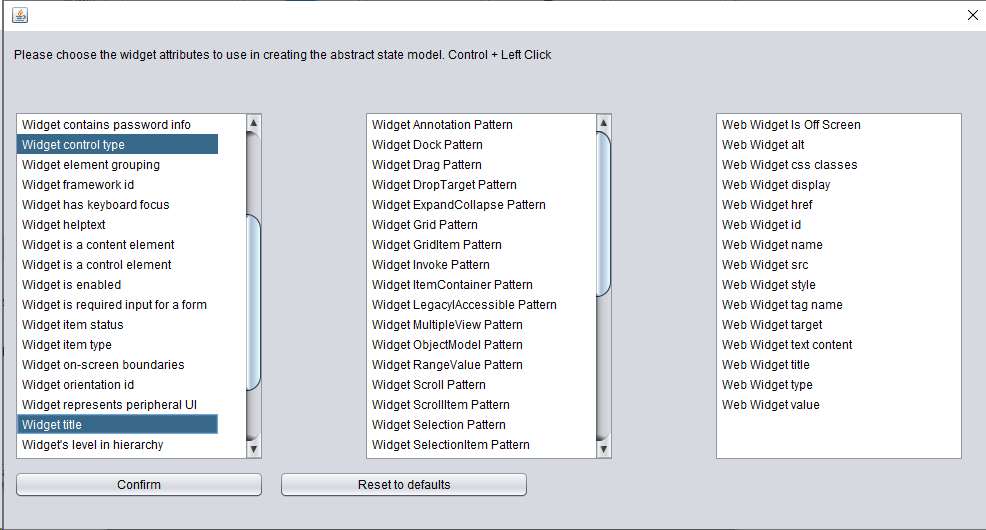
\includegraphics[scale=0.5]{pics/attributes-state-model.png}
\captionof{figure}{Select widgets attributes for the abstractStateId}\label{fig:advance}
\endgroup

Using the \verb|abstractStateId| is excellent for the proof of concept and preliminary change detection, but due to the boolean nature of this comparison, the state either exists or not, it can result in many 'false' changes.

The use of the \verb|abstractStateId| makes it vital to choose sufficient widget attributes. Choosing too few attributes could result in conflicting differences, like the same actions are removed and added. Choosing too many attributes could trigger a change in even the tiniest detail, which can be helpful. Choosing the widget attributes can be done with the 'Advance' screen under the State model tab, see Figure \ref{fig:advance}.

An experiment application is created to discover what the best setting can be. Figure \ref{fig:exp-v1}, \ref{fig:exp-v2} and \ref{fig:exp-v3} shows the three different version of the experiment application. As one can observe, the differences between version 1 and version 2 are the added button with the label 'Hello v2' and between version 2 and 3 the buttons' colour and position. However, when using 'widget title' and 'widget control type' as widget attributes for the abstract state model, a different result is displayed. Namely: between the first two versions, the button with the label 'Hello v1' is removed, and the buttons with the labels 'Hello v1' and 'Hello v2' are added. Between versions 2 and 3, no differences are observed.

\begingroup
\captionsetup{type=figure}
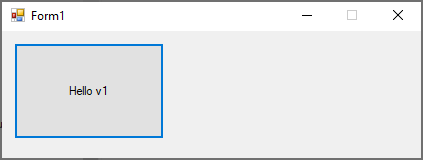
\includegraphics[scale=1]{pics/exp-v1.png}
\captionof{figure}{Version 1 of the experiment application}\label{fig:exp-v1}
\endgroup

\begingroup
\captionsetup{type=figure}
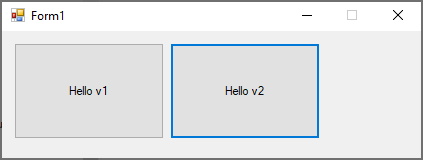
\includegraphics[scale=1]{pics/exp-v2.png}
\captionof{figure}{Version 2 of the experiment application}\label{fig:exp-v2}
\endgroup

\begingroup
\captionsetup{type=figure}
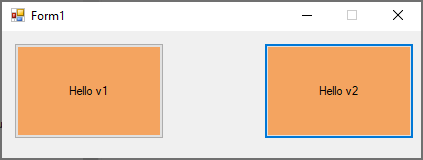
\includegraphics[scale=1]{pics/exp-v3.png}
\captionof{figure}{Version 3 of the experiment application}\label{fig:exp-v3}
\endgroup

When looking at the three versions, it raises interesting questions; 

What are interesting changes? 

Which attributes needs to be taking into account for the \verb|abstractStateId|? 

Might it be of more interest to look into the actions instead of the state? 

Can we leverage image recognition, like with the Murphy tool \cite{murphy-extract-gui}, next to action differences? 

Can it be helpful to make hashes of combined hashes to discover changes or look deeper into underlying hashes, like in a Merkle tree \cite{merkle-tree} structure?

\subsection{TESTAR in containers}
A recent master thesis by Slomp explains how TESTAR can be integrated into a \acrfull{ci} environment. He showed integration with Azure DevOps and introduced TESTAR into the world of Docker and containers. A container bundles all the software, configuration files and libraries together so that an application can run \cite{ms-container}. 

When TESTAR is being run within the Azure DevOps pipeline, the TESTAR GUI is not shown. It is not a problem, but it could be an issue when all the users need to install the TESTAR tool to open the analysis.  